%%%%%%%%%%%%%%%%%%%%%%%%
%% Sample use of the infthesis class to prepare a thesis. This can be used as
%% a template to produce your own thesis.
%%
%% The title, abstract and so on are taken from Martin Reddy's csthesis class
%% documentation.
%%
%% Original template: MEF, October 2002
%% Enhanced template: Yeqi Huang <yeqi.huang@ed.ac.uk>, September 2025
%%   - Added symmetric layout support
%%   - Added phdannual option for annual reviews
%%   - Added multi-disciplinary institute support
%%   - Enhanced template generalization
%%
%% This template builds upon the excellent work by Daniel Hillerstroem,
%% Chris Vasiladiotis, and Laurie Burchell from the CDT in NLP thesis template:
%% https://www.overleaf.com/latex/templates/cdt-in-nlp-thesis/dwhtbkzqpjwx
%% We acknowledge their contributions and have extended their work with
%% additional features including advanced TikZ diagrams, pseudocode examples,
%% enhanced table formatting, and improved citation management.
%%%%%%%%%%%%%%%%%%%%%%%%

%%%%
%% Load the class. Put any options that you want here (see the documentation
%% for the list of options). The following are samples for each type of
%% document:
%%
%% Document types:
%%  phd: PhD thesis (default)
%%  phdannual: PhD annual review
%%  phdproposal: PhD proposal
%%  mphil: Master of Philosophy thesis
%%  mscres: Master of Science by Research
%%  msc: Master of Science taught degree
%%  minf: Master of Informatics
%%  bsc: Bachelor of Science project report
%%
%% Note: you can also specify any of the following options:
%%  logo: put a University of Edinburgh logo onto the title page
%%  frontabs: put the abstract onto the title page
%%  deptreport: produce a title page that fits into a Computer Science
%%      departmental cover [not sure if this actually works]
%%  singlespacing, fullspacing, doublespacing: choose line spacing
%%  oneside, twoside: specify a one-sided or two-sided thesis
%%  10pt, 11pt, 12pt: choose a font size
%%  centrechapter, leftchapter, rightchapter: alignment of chapter headings
%%  sansheadings, normalheadings: headings and captions in sans-serif
%%      (default) or in the same font as the rest of the thesis
%%  [no]listsintoc: put list of figures/tables in table of contents (default:
%%      not)
%%  romanprepages, plainprepages: number the preliminary pages with Roman
%%      numerals (default) or consecutively with the rest of the thesis
%%  parskip: don't indent paragraphs, put a blank line between instead
%%  abbrevs: define a list of useful abbreviations (see documentation)
%%  draft: produce a single-spaced, double-sided thesis with narrow margins
%%
%% For PhD documents -- you must also specify a research institute:
%% Change the first option below to match your document type and institute
\documentclass[phd,ilcc,oneside,logo]{infthesis}
%% For annual review, use: \documentclass[phdannual,ilcc,oneside,logo]{infthesis}
%% For PhD proposal, use: \documentclass[phdproposal,ilcc,oneside,logo]{infthesis}
%%
%% Available institutes/schools:
%% School of Informatics: aiai, cisa, icsa, ianc, ilcc, ipab, lfcs
%% School of Mathematics: maxwell, mathstats
%% School of Physics and Astronomy: physics, astronomy, particle
%% School of Biological Sciences: biology, molcell, ecology
%% School of Chemistry: chemistry
%% School of GeoSciences: geosciences, geology, geography
%%
%% Examples:
%% Mathematics PhD: \documentclass[phd,maxwell,oneside,logo]{infthesis}
%% Physics PhD: \documentclass[phd,physics,oneside,logo]{infthesis}
%% Biology PhD: \documentclass[phd,biology,oneside,logo]{infthesis}
%% Chemistry PhD: \documentclass[phd,chemistry,oneside,logo]{infthesis}

\usepackage[T1]{fontenc}
\usepackage{natbib}
\usepackage[british]{babel}
\usepackage{graphicx}
\usepackage{amsmath,amsfonts,amssymb}  % for maths
\usepackage{booktabs}  % for pretty lines in tables
\usepackage{nth}  % for easy ordinals
\usepackage{csquotes}
\usepackage[colorlinks=true,linkcolor=black,anchorcolor=black,citecolor=black,filecolor=black,menucolor=black,runcolor=black,urlcolor=black]{hyperref}  % for urls
\usepackage{cleveref} % for references to sections/figures/tables...

% Packages for advanced features
\usepackage{algorithm}  % for algorithm environment
\usepackage{algorithmic}  % for pseudocode
\usepackage{tikz}  % for TikZ diagrams
\usetikzlibrary{shapes,arrows,positioning,trees}  % TikZ libraries
\usepackage{pgfplots}  % for plots
\pgfplotsset{compat=1.18}
\usepackage{longtable}  % for long tables
\usepackage{array}  % for enhanced table features
\usepackage{multirow}  % for multirow cells in tables

%% Information about the title, etc.
%% Change these to match your document
\title{Your Document Title}
\author{Your Name Here}

%% If the year of submission is not the current year, uncomment this line and
%% specify it here:
%\submityear{2025}

%% Optionally, specify the graduation month and year:
%\graduationdate{June 2025}

%% Specify the abstract here.
\abstract{
This enhanced University of Edinburgh thesis template builds upon the excellent
work by Daniel Hillerstroem, Chris Vasiladiotis, and Laurie Burchell from their
CDT in NLP thesis template (https://www.overleaf.com/latex/templates/cdt-in-nlp-thesis/dwhtbkzqpjwx).

This template extends the original work with additional features including:
comprehensive pseudocode examples using the algorithm and algorithmic packages,
advanced TikZ diagrams for flowcharts and mathematical visualizations,
enhanced table formatting with support for complex multi-row and multi-column layouts,
improved citation management with multiple reference styles,
and optional supervisor signature sections for different institutional requirements.

The template maintains compatibility with the original infthesis class while
providing modern LaTeX best practices and extensive documentation through
example chapters that demonstrate all available features.
}

%% Now we start with the actual document.
\begin{document}

%% First, the preliminary pages
\begin{preliminary}

%% This creates the title page
\maketitle

% Lay summary
\cleardoublepage
\begin{center}
\textsf{\textbf{Summary}}
\end{center}
Lay summary here

\cleardoublepage

%% Acknowledgements
\begin{acknowledgements}
Acknowledgements here
\end{acknowledgements}

%% Next we need to have the declaration.
\standarddeclaration

%% Finally, a dedication (this is optional -- uncomment the following line if
%% you want one).
% \dedication{}

%% Create the table of contents
\tableofcontents

%% If you want a list of figures or tables, uncomment the appropriate line(s)
% \listoffigures
% \listoftables

\end{preliminary}

%%%%%%%%
%% Include your chapter files here. See the sample chapter file for the basic
%% format.

% chapters start like this. You can refer to them using the label like this: \cref{ch:intro}
\chapter{Introduction}
\label{ch:intro}

This is an example chapter. You cite like this: \cite{burchell-etal-2023-open}. \Cref{fig:tiredwired} shows an example of a figure.

\begin{figure}[htbp]
    \centering
    
\includegraphics[width=0.9\linewidth]{figures/tiredwired.png}
    \caption{This is an example figure.}
    \label{fig:tiredwired}
\end{figure}
\chapter{Advanced Features Examples}
\label{chap:examples}

This chapter demonstrates various advanced features commonly used in academic theses, including pseudocode algorithms, TikZ diagrams, complex tables, and proper citation formatting.

\section{Lorem Ipsum Overview}

Lorem ipsum dolor sit amet, consectetur adipiscing elit. Sed do eiusmod tempor incididunt ut labore et dolore magna aliqua. Ut enim ad minim veniam, quis nostrud exercitation ullamco laboris \citep{knuth1984texbook}. Excepteur sint occaecat cupidatat non proident, sunt in culpa qui officia deserunt mollit anim id est laborum.

Duis aute irure dolor in reprehenderit in voluptate velit esse cillum dolore eu fugiat nulla pariatur. This methodology has been widely adopted in recent research \cite{lamport1986latex}.

\section{Pseudocode Examples}

Algorithm design is a fundamental aspect of computer science research. \Cref{alg:quicksort} presents the classic QuickSort algorithm in pseudocode format.

\begin{algorithm}
\caption{QuickSort Algorithm}
\label{alg:quicksort}
\begin{algorithmic}[1]
\REQUIRE Array $A[1..n]$ of comparable elements
\ENSURE Array $A$ sorted in non-decreasing order
\STATE \textbf{function} QuickSort($A$, $low$, $high$)
\IF{$low < high$}
    \STATE $pivot \leftarrow$ Partition($A$, $low$, $high$)
    \STATE QuickSort($A$, $low$, $pivot - 1$)
    \STATE QuickSort($A$, $pivot + 1$, $high$)
\ENDIF
\STATE \textbf{end function}
\end{algorithmic}
\end{algorithm}

Lorem ipsum dolor sit amet, consectetur adipiscing elit. The time complexity of QuickSort is $O(n \log n)$ on average, making it highly efficient for large datasets \citep{cormen2009introduction}.

\begin{algorithm}
\caption{Binary Search}
\label{alg:binarysearch}
\begin{algorithmic}[1]
\REQUIRE Sorted array $A[1..n]$, target value $x$
\ENSURE Index of $x$ in $A$, or $-1$ if not found
\STATE $left \leftarrow 1$
\STATE $right \leftarrow n$
\WHILE{$left \leq right$}
    \STATE $mid \leftarrow \lfloor (left + right) / 2 \rfloor$
    \IF{$A[mid] = x$}
        \RETURN $mid$
    \ELSIF{$A[mid] < x$}
        \STATE $left \leftarrow mid + 1$
    \ELSE
        \STATE $right \leftarrow mid - 1$
    \ENDIF
\ENDWHILE
\RETURN $-1$
\end{algorithmic}
\end{algorithm}

\section{TikZ Diagrams and Visualizations}

Visual representations are crucial for explaining complex concepts. \Cref{fig:flowchart} shows a simple flowchart created using TikZ.

\begin{figure}[htbp]
\centering
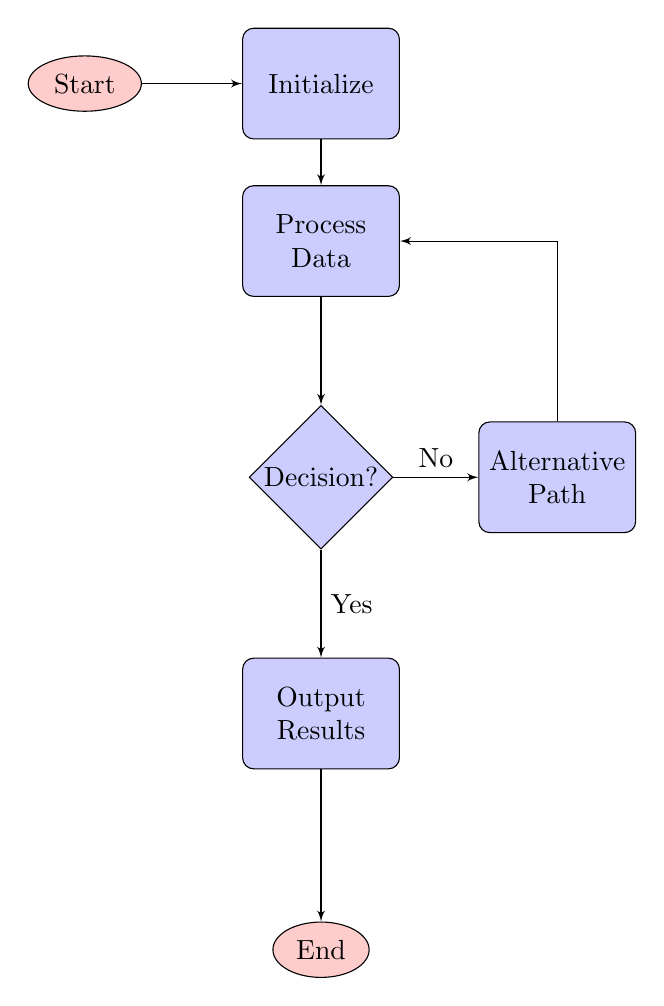
\begin{tikzpicture}[node distance=2cm, auto]
    % Define styles
    \tikzstyle{decision} = [diamond, draw, fill=blue!20,
        text width=4.5em, text badly centered, node distance=3cm, inner sep=0pt]
    \tikzstyle{block} = [rectangle, draw, fill=blue!20,
        text width=5em, text centered, rounded corners, minimum height=4em]
    \tikzstyle{line} = [draw, -latex']
    \tikzstyle{cloud} = [draw, ellipse, fill=red!20, node distance=3cm,
        minimum height=2em]

    % Place nodes
    \node [block] (init) {Initialize};
    \node [cloud, left of=init] (start) {Start};
    \node [block, below of=init] (process) {Process Data};
    \node [decision, below of=process] (decide) {Decision?};
    \node [block, below of=decide, node distance=3cm] (output) {Output Results};
    \node [cloud, below of=output] (end) {End};
    \node [block, right of=decide, node distance=3cm] (alternative) {Alternative Path};

    % Draw edges
    \path [line] (start) -- (init);
    \path [line] (init) -- (process);
    \path [line] (process) -- (decide);
    \path [line] (decide) -- node {Yes} (output);
    \path [line] (decide) -- node {No} (alternative);
    \path [line] (alternative) |- (process);
    \path [line] (output) -- (end);
\end{tikzpicture}
\caption{Example flowchart demonstrating TikZ capabilities}
\label{fig:flowchart}
\end{figure}

Sed ut perspiciatis unde omnis iste natus error sit voluptatem accusantium doloremque laudantium. \Cref{fig:tree} illustrates a binary tree structure.

\begin{figure}[htbp]
\centering
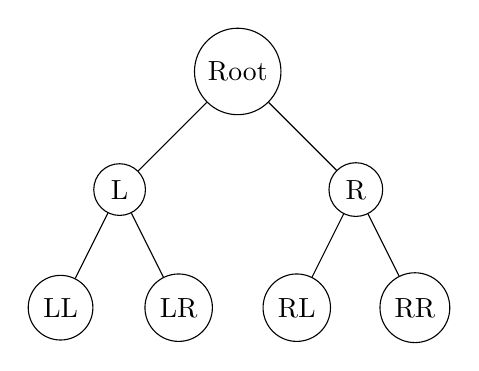
\begin{tikzpicture}[level distance=1.5cm,
  level 1/.style={sibling distance=3cm},
  level 2/.style={sibling distance=1.5cm}]
  \node [circle,draw] {Root}
    child {node [circle,draw] {L}
      child {node [circle,draw] {LL}}
      child {node [circle,draw] {LR}}
    }
    child {node [circle,draw] {R}
      child {node [circle,draw] {RL}}
      child {node [circle,draw] {RR}}
    };
\end{tikzpicture}
\caption{Binary tree visualization using TikZ}
\label{fig:tree}
\end{figure}

\section{Mathematical Plots}

Data visualization is essential for presenting research findings. \Cref{fig:plot} shows a mathematical function plot.

\begin{figure}[htbp]
\centering
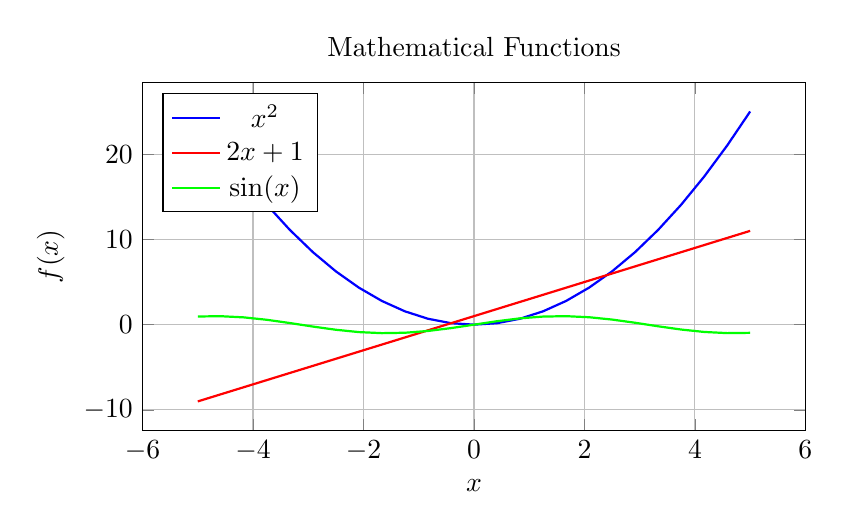
\begin{tikzpicture}
\begin{axis}[
    xlabel={$x$},
    ylabel={$f(x)$},
    title={Mathematical Functions},
    legend pos=north west,
    grid=major,
    width=10cm,
    height=6cm
]
\addplot[blue, thick] {x^2};
\addplot[red, thick] {2*x + 1};
\addplot[green, thick] {sin(deg(x))};
\legend{$x^2$, $2x+1$, $\sin(x)$}
\end{axis}
\end{tikzpicture}
\caption{Example mathematical functions plotted using PGFPlots}
\label{fig:plot}
\end{figure}

\section{Advanced Table Examples}

Tables are fundamental for presenting structured data. \Cref{tab:simple} shows a basic comparison table.

\begin{table}[htbp]
\centering
\caption{Performance comparison of different algorithms}
\label{tab:simple}
\begin{tabular}{@{}lccr@{}}
\toprule
Algorithm & Time Complexity & Space Complexity & Stability \\
\midrule
QuickSort & $O(n \log n)$ & $O(\log n)$ & No \\
MergeSort & $O(n \log n)$ & $O(n)$ & Yes \\
HeapSort & $O(n \log n)$ & $O(1)$ & No \\
BubbleSort & $O(n^2)$ & $O(1)$ & Yes \\
\bottomrule
\end{tabular}
\end{table}

Lorem ipsum dolor sit amet, consectetur adipiscing elit, sed do eiusmod tempor incididunt ut labore et dolore magna aliqua. For more complex data presentations, \Cref{tab:complex} demonstrates advanced table features.

\begin{table}[htbp]
\centering
\caption{Complex table with multirow and multicolumn cells}
\label{tab:complex}
\begin{tabular}{@{}lcccc@{}}
\toprule
\multirow{2}{*}{Dataset} & \multicolumn{2}{c}{Training} & \multicolumn{2}{c}{Testing} \\
\cmidrule(lr){2-3} \cmidrule(lr){4-5}
& Accuracy & F1-Score & Accuracy & F1-Score \\
\midrule
MNIST & 98.5\% & 0.985 & 97.8\% & 0.978 \\
CIFAR-10 & 85.2\% & 0.851 & 82.1\% & 0.820 \\
ImageNet & 76.3\% & 0.762 & 73.9\% & 0.738 \\
\multirow{2}{*}{Custom} & 91.7\% & 0.916 & 89.4\% & 0.893 \\
& (Subset A) & & (Subset A) & \\
\bottomrule
\end{tabular}
\end{table}

\section{Long Table Example}

For tables that span multiple pages, the \texttt{longtable} environment is useful:

\begin{longtable}{@{}lp{3cm}p{3cm}p{3cm}@{}}
\caption{Experimental results across multiple conditions} \label{tab:long} \\
\toprule
Condition & Method A & Method B & Method C \\
\midrule
\endfirsthead

\multicolumn{4}{c}%
{{\bfseries \tablename\ \thetable{} -- continued from previous page}} \\
\toprule
Condition & Method A & Method B & Method C \\
\midrule
\endhead

\midrule \multicolumn{4}{r}{{Continued on next page}} \\
\endfoot

\bottomrule
\endlastfoot

Condition 1 & Lorem ipsum dolor sit amet & Consectetur adipiscing elit & Sed do eiusmod tempor \\
Condition 2 & Ut labore et dolore magna & Quis nostrud exercitation & Ullamco laboris nisi \\
Condition 3 & Duis aute irure dolor & Excepteur sint occaecat & Cupidatat non proident \\
Condition 4 & Sunt in culpa qui officia & Mollit anim id est & Laborum sed ut \\
Condition 5 & Perspiciatis unde omnis & Iste natus error sit & Voluptatem accusantium \\
Condition 6 & Doloremque laudantium & Totam rem aperiam & Eaque ipsa quae \\
Condition 7 & Ab illo inventore & Veritatis et quasi & Architecto beatae vitae \\
Condition 8 & Dicta sunt explicabo & Nemo enim ipsam & Voluptatem quia voluptas \\
\end{longtable}

\section{Citations and References}

Proper citation is crucial in academic writing. This section demonstrates various citation styles:

\begin{itemize}
\item Single citation: \cite{knuth1984texbook}
\item Multiple citations: \cite{lamport1986latex,cormen2009introduction}
\item Parenthetical citation: \citep{knuth1984texbook}
\item Textual citation: \citet{lamport1986latex} introduced the LaTeX document preparation system
\item Citation with page numbers: \citep[p.~42]{cormen2009introduction}
\item Citation with prenote and postnote: \citep[see][Chapter 3]{knuth1984texbook}
\end{itemize}

Lorem ipsum dolor sit amet, consectetur adipiscing elit. Recent advances in machine learning \citep{cormen2009introduction} have shown significant improvements in various domains. The foundational work by \citet{knuth1984texbook} established many of the principles still used today.

Sed ut perspiciatis unde omnis iste natus error sit voluptatem accusantium doloremque laudantium, totam rem aperiam, eaque ipsa quae ab illo inventore veritatis et quasi architecto beatae vitae dicta sunt explicabo.

\section{Cross-References}

LaTeX provides excellent cross-referencing capabilities using the \texttt{cleveref} package:

\begin{itemize}
\item Reference to chapter: \Cref{chap:examples}
\item Reference to section: \Cref{sec:conclusions} (in next section)
\item Reference to figure: \Cref{fig:flowchart,fig:tree}
\item Reference to table: \Cref{tab:simple,tab:complex}
\item Reference to algorithm: \Cref{alg:quicksort,alg:binarysearch}
\item Reference to equation: \Cref{eq:example} below
\end{itemize}

The quadratic formula is given by:
\begin{equation}
x = \frac{-b \pm \sqrt{b^2 - 4ac}}{2a}
\label{eq:example}
\end{equation}

\section{Conclusions}
\label{sec:conclusions}

This chapter has demonstrated the key features available in this thesis template:

\begin{enumerate}
\item Pseudocode algorithms using the \texttt{algorithm} and \texttt{algorithmic} packages
\item TikZ diagrams for flowcharts, trees, and mathematical plots
\item Simple and complex tables with the \texttt{booktabs} package
\item Long tables that can span multiple pages
\item Proper citation formatting using \texttt{natbib}
\item Cross-referencing with \texttt{cleveref}
\end{enumerate}

Lorem ipsum dolor sit amet, consectetur adipiscing elit, sed do eiusmod tempor incididunt ut labore et dolore magna aliqua. These tools provide a comprehensive foundation for creating professional academic documents.

%%%%%%%%
%% Any appendices should go here. The appendix files should look just like the
%% chapter files.
%\appendix
%\include{chapters/99appendix}

%% Choose your favourite bibliography style here.
\bibliographystyle{apalike}

%% If you want the bibliography single-spaced (which is allowed), uncomment
%% the next line.
%\singlespace

\bibliography{anthology}

\end{document}
